% !TEX encoding = UTF-8 Unicode
\chapter{Trabajos Relacionados} 
Hace relativamente poco tiempo que se empezaron a utilizar las Unidades de Medición Inerciales o IMU (Inertial Measurement Unit, por sus siglas en inglés).
El principal uso que se les daba cuando aún no eran tan conocidas, fue utilizarlas como herramienta para fines de investigación científica; principalmente en el campo de la robótica o en la industria aeroespacial, mejorando los sistemas de navegación. 
Sin embargo, debido a: el auge que las tecnologías de la información han tenido en los últimos años, el mejoramiento en la precisión de las mediciones de los dispositivos, así como el gran número de innovaciones tecnológicas que han surgido, es que estas piezas tecnológicas han encontrado un sinfín de aplicaciones. 
Tal es el caso, que en la actualidad la gran mayoría de los teléfonos móviles cuentan con este tipo de sensores.

El aspecto del perfeccionamiento de las IMU’s es un tema en el que la investigación no ha dejado de enfocarse para ofrecer un mejor rendimiento a la hora de hacer uso de estas, y por ende, mejores resultados en los diferentes ámbitos en los que se les utiliza. 
Tal es el caso de \cite{768189}, donde los autores tratan de corregir los errores intrínsecos en las mediciones de las IMU y el GPS, a través de la implementación de técnicas de detección de fallas en sistemas de navegación de vehículos autónomos terrestres; tales como sesgos en las lecturas de los sensores y desalineaciones (llamados errores de baja frecuencia) ambas por parte de las IMU’s, y errores de posicionamiento por parte de los GPS’s (llamados errores de alta frecuencia). 
Esto lo hacen con el objetivo de lograr una mayor integridad en sistemas autónomos terrestres; y por ende, conseguir una mayor autonomía y robustez en la navegación.

%\textcolor{blue}{
Otras investigaciones se centran en mejorar la eficiencia de dispositivos, tales como los receptores GPS, con el fin de lograr una mejor precisión en el posicionamiento del vehículo.
%} \textcolor{red}{no entiendo eso de auxiliar a otros dispositivos}
Por ejemplo, en \cite{NAVI:NAVI403} se busca minimizar los errores de posicionamiento del GPS en vehículos a través de actualizaciones de velocidad auxiliares dadas por IMU, usando herramientas como el Filtro de Kalman Extendido, entre otras. 
Los autores buscan resolver la problemática que presentan hoy en día los GPS en cuestión de precisión y pérdidas de conexión por bloqueo de señal en áreas urbanas.
Su solución es barata debido al bajo costo de los IMU.

En la figura \ref{NAVI} se muestra la disminución en los errores de posición conseguida.

%\begin{figure}[H]
%\centering
%a)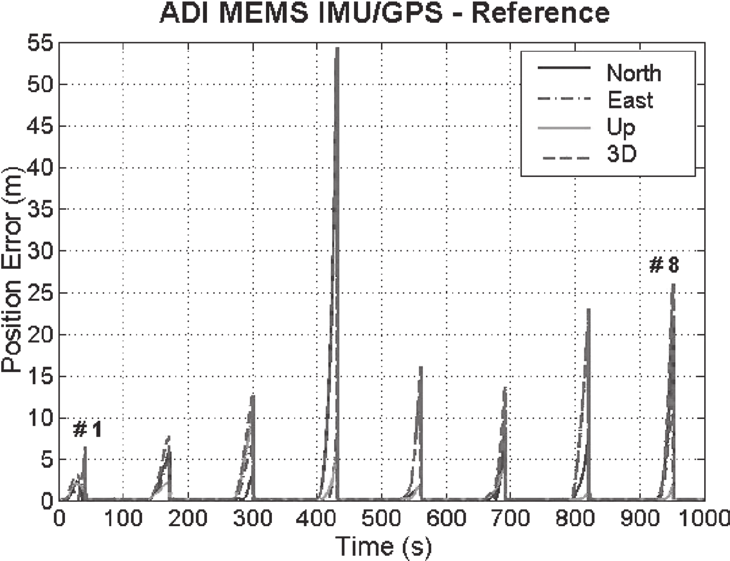
\includegraphics[scale=.2]{2a.png}b)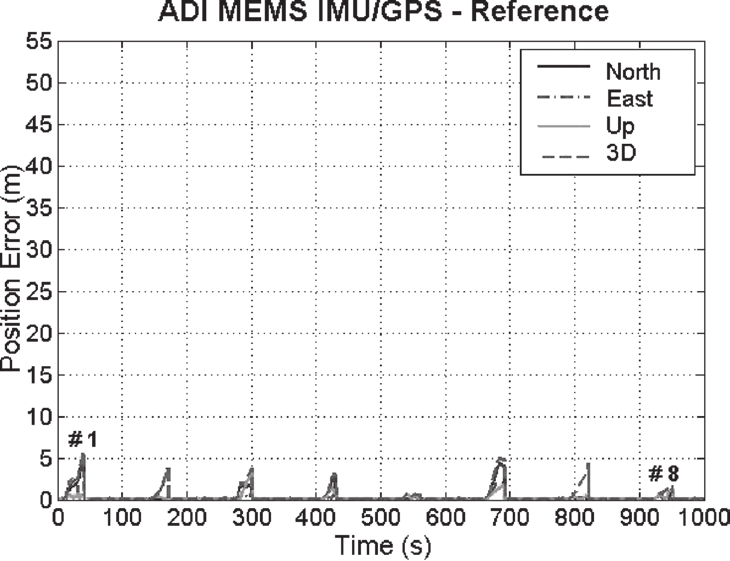
\includegraphics[scale=.2]{2b.png}
%\caption{2 b}
%\end{figure}

\begin{figure}[H]
\begin{tikzpicture}
\centering
  \node[inner sep=0pt] (A) {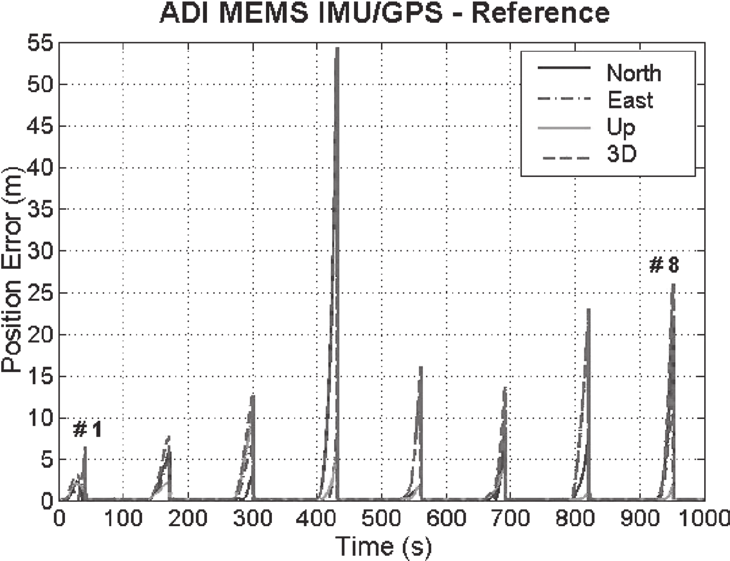
\includegraphics[scale=0.28]{2a.png}\hspace{1cm}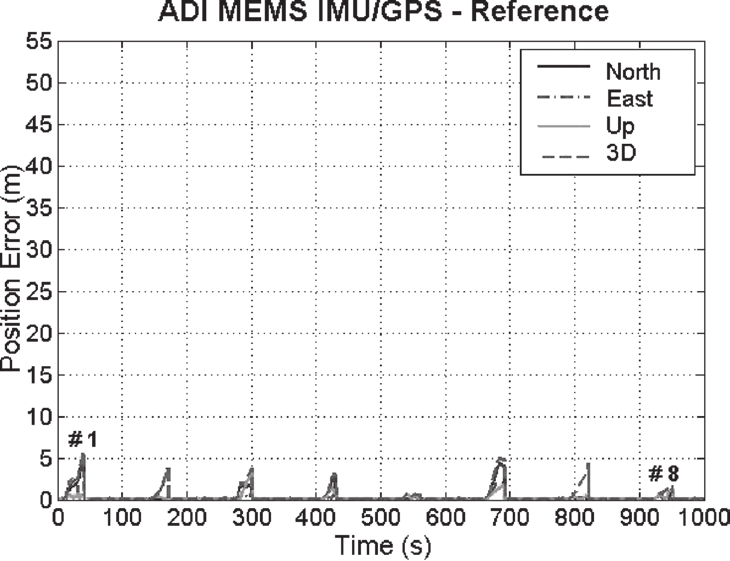
\includegraphics[scale=.28]{2b.png}};
  \node at (-4,-3.4) {$a)$};
  \node at (4,-3.4) {$b)$};
%  \node at (7.7,4.1) {\small #2};
\end{tikzpicture}
\caption{$a)$ Errores de posición durante periodos sin conexión GPS. $b)$ Errores de posición durante periodos sin conexión GPS aplicando actualizaciones auxiliares (imagen tomada de \cite{NAVI:NAVI403}).}
\label{NAVI}
\end{figure}

La integración de IMU’s en los teléfonos móviles es el caso más conocido de la aplicación de estos sensores en la vida cotidiana. 
Sin embargo existen muchas otras aplicaciones, que si bien no son tan masivas y conocidas como el caso de los teléfonos móviles, ayudan a pequeños sectores de la población y de la industria a realizar tareas más eficientemente. 
Como un ejemplo de ello se puede mencionar a los drones, para los cuales este tipo de sensores es indispensable para su correcto funcionamiento \cite{6852167}.

Aún con todas las implementaciones de los sensores de aceleración, todavía existen infinitas posibilidades de aplicación para esta tecnología. 
Por lo que se puede decir que los beneficios directos e indirectos de su uso están aún, en su mayoría, a la espera de que nuevas aplicaciones sean descubiertas y desarrolladas.
 
Muchas de estas aplicaciones ya se están elaborando hoy en día y el espectro de disciplinas en las que podrían aprovecharse sus beneficios es bastante amplio. 
Tal es el ejemplo de los trabajos realizados en \cite{7457644}, donde se hace uso de las IMU’s para activar el motor de bicicletas eléctricas, al detectar mediante estos sensores cuando el usuario conduce en la bicicleta.
También se realiza un análisis del comportamiento de la dinámica de la bicicleta para determinar si el movimiento de esta, corresponde a un desplazamiento común cuando el usuario la va manejando, a un desplazamiento donde el usuario va caminando con ella o a un movimiento accidental del pedal; con el fin de que no se active el motor en estos dos últimos casos.  

\begin{figure}[H]
\centering
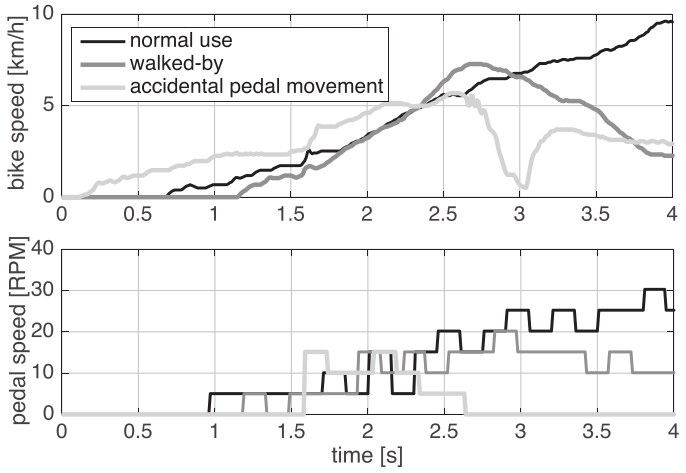
\includegraphics[scale=0.7]{3.png}
\caption{Velocidad de la bicicleta (medida a través de la velocidad del motor) y ritmo del pedal. Se presentan tres eventos diferentes: pedaleo normal, caminar con la bicicleta y movimiento accidental del pedal (imagen tomada de \cite{7457644}).} 
\label{3}
\end{figure}

Otra aplicación interesante de estos dispositivos en medios de transporte es la que se describe en \cite{7072991}. El principal objetivo de este trabajo es la detección de desalineaciones en vías de tren. 
Lo cual se lleva a cabo colocando un sensor inercial dentro de un tren y aplicando la teoría del análisis de Fourier a sus mediciones, con el fin de analizar los espectros de frecuencias y encontrar así posibles desalineaciones. 
Además de que, con este mismo análisis se detecta ruido proveniente del motor y la suspensión del tren. 
Sus beneficios son una mejor identificación de potenciales desalineaciones y su bajo costo en la detección. \\

\begin{figure}[H]
\centering
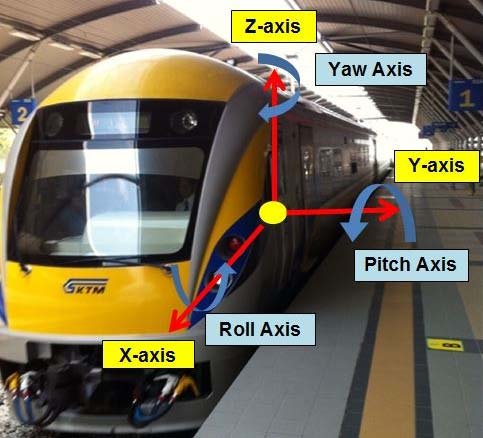
\includegraphics[scale=0.5]{4.png}
\caption{Sistema ejes de los tres ángulos de Euler y ejes de aceleración en el tren (imagen tomada de \cite{7072991}).}
\label{4}
\end{figure}

Análogo al trabajo desarrollado en \cite{7072991} es el proyecto que se expone en \cite{Seraj:2015:SBM:2800835.2800981}, donde en lugar de brindar soluciones para la detección de anomalías producidas en vías férreas, se busca hacer lo equivalente en las autopistas. 
Para esto se hace uso de los sensores integrados en los teléfonos móviles con el fin de recolectar información de la dinámica de un vehículo. 
Esta información es usada para la detección de curvas en el camino, mediante el cálculo del ángulo de desviación del vehículo al dar vuelta. 
Además, con el método implementado se distingue entre distintos eventos de comportamiento de un conductor, al analizar la dinámica del vehículo. 
La detección de anomalías en el camino es lograda al estudiar las características de las curvas, utilizando técnicas como el aprendizaje automático y la Transformada Ondeleta (o Wavelet) Estacionaria.

Otros proyectos orientados a proporcionar soluciones para vehículos, como es el caso del presente trabajo, se enfocan en diferentes cuestiones, las cuales no están necesariamente ligadas a la dinámica del vehículo; tal es el caso de \cite{Quito}.
En este proyecto se tiene el objetivo de identificar y reparar las fuentes de vibración de vehículos pequeños, mediante el uso de la teoría de vibraciones. 
Los autores hacen uso de un analizador (figura \ref{5}), el cual es un aparato que usa la transformada rápida de Fourier para identificar las vibraciones del vehículo; esto se logra colocando el aparato dentro del vehículo y realizando las pruebas correspondientes. 
El dispositivo proporciona información sobre las causas de las vibraciones en vehículos en los que se realizan las pruebas. 
Todo lo anterior con el fin de reducir la molestia de los usuarios por motivos de estas vibraciones, así como a través de este análisis, saber cuando el vehículo se encuentra en mal estado.

\begin{figure}[H]
\centering
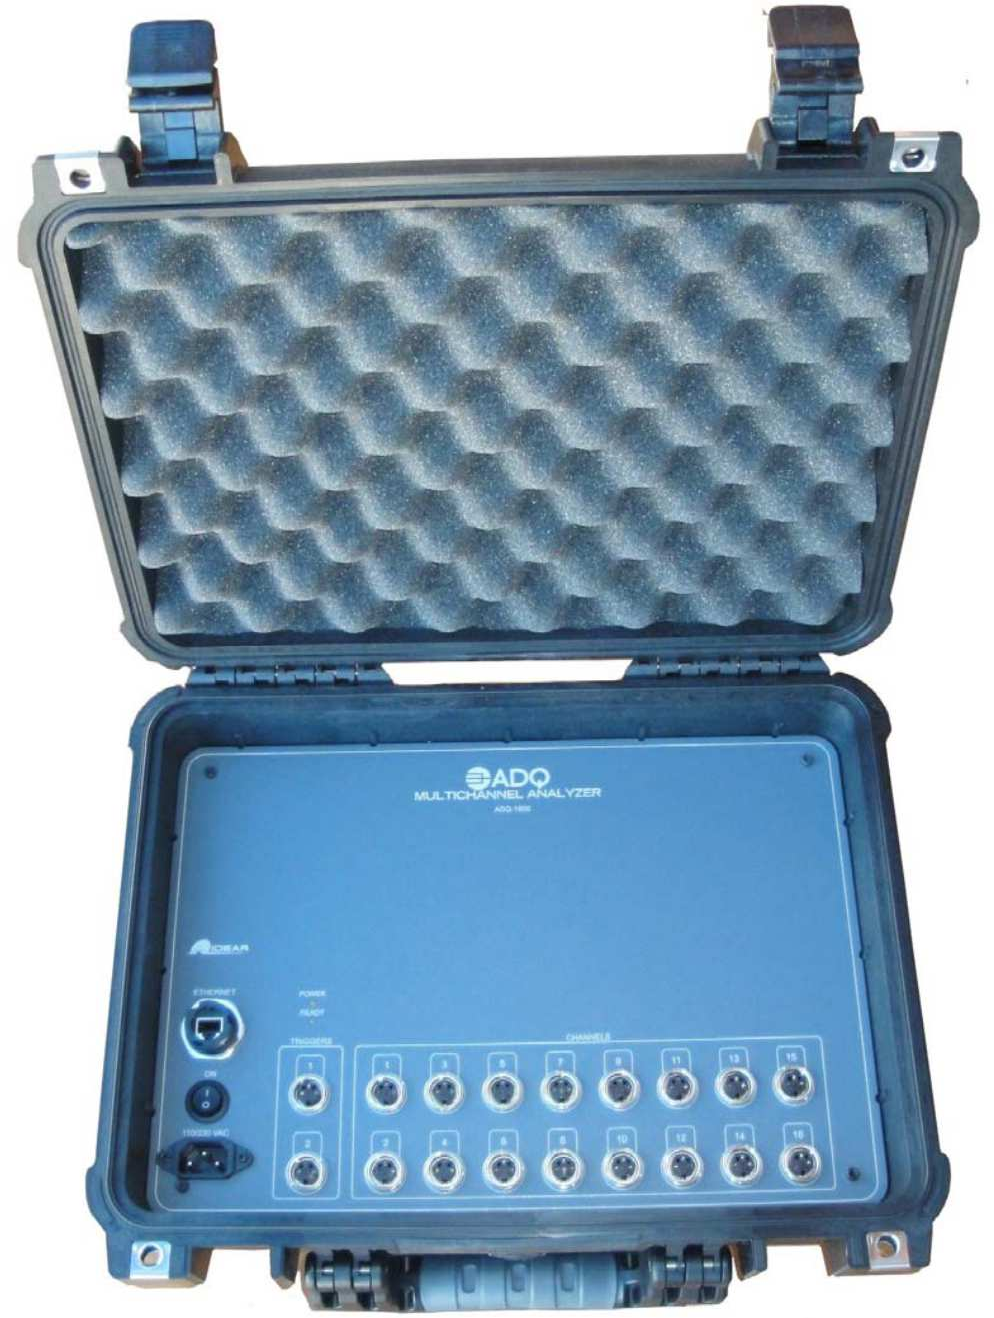
\includegraphics[scale=0.4]{5.png}
\caption{Analizador (imagen tomada de \cite{Quito}).}
\label{5}
\end{figure}

%Además de las metodologías empleadas en este trabajo para la identificación de maniobras anómalas en la conducción de vehículos, existen también otras opciones que ofrecen la solución a esta misma problemática, pero con técnicas muy diferentes a las del análisis espectral o el análisis de la dinámica del vehículo. 
Para dar solución a la problematica descrita en el presente trabajo de tesis existen diferentes técnicas y metodologías.
Una recopilación de varias técnicas para la detección de comportamientos en conductores de automóviles, tales como somnolencia, distracción, ojos cerrados, entre otros, es presentada en \cite{7225158}.
Dentro de estas técnicas, una de las más interesantes es el análisis de imágenes digitales para la detección de los comportamientos mencionados. 
La cual consiste en la colocación de una cámara en el vehículo, de forma tal que, obtenga imágenes del rostro del conductor; para posteriormente, mediante un algoritmo implementado por una computadora, detectar las características de somnolencia, ojos cerrados, etc. 
Otra de las técnicas utilizadas para detectar la fatiga y somnolencia de los conductores es la implementación de análisis psicológicos. 
Con esto se tiene la intención de medir ciertos parámetros físicos y psicológicos, a través de electroencefalogramas y mediciones del ritmo cardiaco del conductor. 
Finalmente, los autores de esta recopilación concluyen diciendo que consideran que cada uno de los métodos que pueden emplearse para la detección de anomalías en la conducción tienen sus pros y contras. 
Por lo que, señalan, la mejor opción es la combinación de varias de estas metodologías.

\begin{figure}[H]
\centering
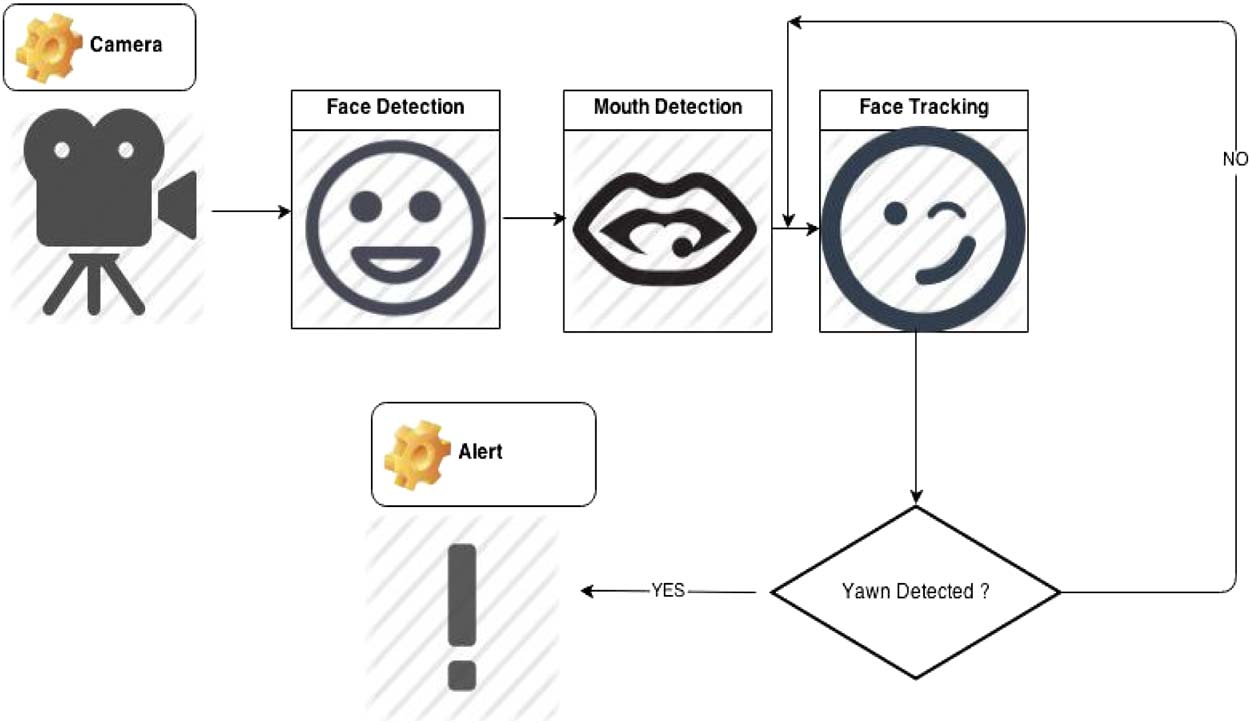
\includegraphics[scale=0.3]{6.png}
\caption{Diagrama de flujo para el análisis de boca y bostezo (imagen tomada de \cite{7225158}).}
\label{6}
\end{figure}


Muchos de los esfuerzos empleados en monitorear la dinámica de un vehículo se centran en el desarrollo de aplicaciones para teléfonos móviles, que ofrezcan información sobre el comportamiento de este a lo largo de alguna trayectoria. 
Uno de los trabajos con estas características es \cite{Valladolid}, donde el principal objetivo de los autores es el análisis de la dinámica del vehículo con fines de detección y prevención de conductas anómalas. 
Su propósito es crear una aplicación móvil que asista al usuario durante la conducción de su vehículo, la cual hace uso de acelerómetros, giroscopios y/o GPS integrados en el teléfono. 
La aplicación que se intenta desarrollar alertará cuando el estilo de conducción sea agresivo mediante sonidos e información en la pantalla del teléfono en tiempo real. 
Buscando siempre que la conducción se haga de manera eficiente.
Mediante el uso del GPS la aplicación mostrará donde se registraron tales eventos de conducción y almacenará la información que se genere durante el trayecto, por ejemplo, datos de aceleración y velocidad en forma gráfica. 
También registrará y mostrará la ruta recorrida mediante la información obtenida por el GPS, señalando los puntos críticos donde se realizaron lo que los autores llaman {\em maniobras agresivas}. 
Se hace un enfoque especial en la detección y posterior aviso de tres eventos de conducción: aceleradas, frenadas y giros. 
La forma de detectar cada uno de los tres diferentes eventos mencionados es a través de umbrales de aceleración y de velocidad angular, por encima de los cuales se considera la realización de alguno de los eventos.

Si bien el uso de teléfonos móviles para el estudio de la dinámica de vehículos tiene un gran potencial, aún existen inconvenientes muy puntuales en el uso de esta tecnología para tales fines.
En \cite{7266726} se busca solucionar el problema de la alineación de los sensores de un teléfono móvil con respecto al vehículo que se pretenda analizar. 
Partiendo de constricciones no holonómicas para la dinámica de un automóvil (como lo es que la velocidad perpendicular a la dirección de movimiento principal del automóvil sea aproximadamente $0$) se busca que la alineación de los sensores quede determinada a lo largo de la navegación del vehículo. 
Actualizándola recursivamente a través del filtro de Kalman, sin la necesidad de una precalibración de los sensores e independientemente de la orientación del teléfono relativa al vehículo.

Otro de los campos de aplicación del análisis de la dinámica de la conducción, aparte de la prevención y alerta de conductas anormales, es la utilización de la información registrada para la deducción de comportamientos del piloto durante la conducción, todo ello con fines legales. 
En \cite{Quito2} se trata de desarrollar un sistema que permita conocer los movimientos y la ruta que ha seguido un vehículo a partir del uso de herramientas tecnológicas como IMU’s y GPS. 
Tal sistema, mostrado en la figura \ref{8}, consiste de una carcasa de metal de $20cm\times 20cm\times 10cm$, la cual contiene el hardware y software necesarios para llevar a cabo los cálculos requeridos para los fines ya mencionados. 
El sistema se conecta a la batería del vehículo, manteniéndolo lo más fijo posible en este para una correcta recopilación de datos. 
Se desea utilizar dicho sistema en la determinación de causas de accidentes de tránsito y localización del vehículo en caso de robo, mediante el análisis de las gráficas de aceleración, velocidad y posición del vehículo que ofrece el dispositivo. 
Para llevar a cabo dicho análisis, en este trabajo los autores realizan pruebas de conducción con el dispositivo a bordo, ejecutando distintas maniobras de prueba con el fin de que los sensores registren su dinámica, tales maniobras se listan a continuación\zsavepos{cont}:
\vspace{8cm}

\begin{textblock*}{\textwidth}(4.7cm,\dimexpr\paperheight-\zposy{cont}sp+5mm)
\begin{itemize}
\item Reposo
\item Conducción normal 
\item Frenado leve 
\item Aceleración rápida 
\item Frenado brusco 
\end{itemize}
\end{textblock*}

\begin{textblock*}{\textwidth}(11.7cm,\dimexpr\paperheight-\zposy{cont}sp+5mm)
\begin{itemize}
\item Camino en mal estado 
\item Aceleración normal 
\item Frenado rápido a fondo
\item Aumento normal de velocidad 
\item Velocidad constante
\end{itemize}
\end{textblock*}

\begin{figure}[H]
\centering
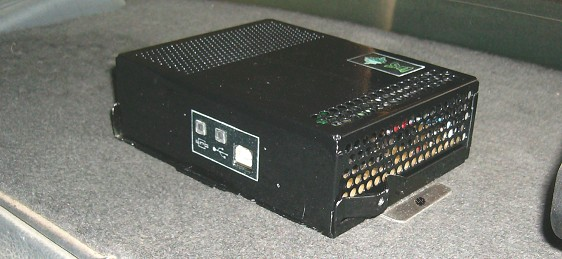
\includegraphics[scale=0.7]{8.png}
\caption{Prototipo instalado en el vehículo (imagen tomada de \cite{Quito2}).}
\label{8}
\end{figure}

Sin embargo, la realización del análisis de las gráficas de aceleración, velocidad y posición generadas en esta prueba solo es de carácter cualitativo.
Ya que los autores únicamente ponen atención a la forma que tienen las diferentes gráficas, para posteriormente deducir si el conductor realizó alguno de los eventos antes mencionados. 

Otra aplicación móvil encaminada a la evaluación del comportamiento de los conductores es la desarrollada en \cite{Paefgen:2012:DBA:2406367.2406412}. 
Donde los autores se basan principalmente en las medidas de aceleración proporcionadas por las IMU’s, así como en información complementaria recibida de otros dispositivos como giroscopios electrónicos y GPS integrados en los teléfonos móviles. 
Esto para detectar lo que ellos llaman eventos críticos de conducción, los cuales se listan a continuación:

\begin{itemize}
\item Aceleración
\item Frenada
\item Vuelta a la izquierda
\item Vuelta a la derecha
\end{itemize}

La detección de estos eventos está basada en la superación de diferentes umbrales de aceleración, correspondientes a cada evento. 
Con la información recabada por el teléfono móvil se pretende dar la correspondiente retroalimentación a los conductores a través de la aplicación; brindándoles información sobre la forma en la que condujeron sus recorridos y añadiéndola a un perfil generado por esta aplicación. 
Cabe mencionar que en este estudio se toma en cuenta el tipo de carretera como factor a considerar en la obtención de datos, característica que no se toma en cuenta muchos otros trabajos relacionados.
Los autores justifican que una aplicación móvil es una mejor opción que una {\em caja negra} (como la que se desarrolla en \cite{Quito2}), ya que, según ellos, tiene una mejor interactividad y permite al usuario tener un mejor acceso y manejo de su información; todo ello con vías a mejorar su comportamiento en la conducción.
Además, mediante el uso de la aplicación se pueden establecer redes sociales que contribuyan a mejorar la seguridad en el tráfico de vehículos.

En \cite{vaiana2014driving} se señala que la seguridad en el tráfico y la eficiencia en el gasto de energía de los vehículos están estrictamente ligados al comportamiento del conductor. 
En este artículo se explica el desarrollo de una aplicación para teléfonos móviles, que pueda evaluar el grado de seguridad que los conductores mantienen al conducir; esto por medio de mediciones de aceleración longitudinal y lateral. 
Para ello se realizan varias pruebas con distintos conductores y vehículos. 
La forma en que se detecta si se está realizando un correcto o incorrecto estilo de conducción es mediante el estudio de las gráficas de aceleración obtenidas, donde se tienen áreas designadas para diferentes formas de conducir. 
La evaluación de la forma de conducir dependerá de la zona de la gráfica donde se registren los datos de aceleraciones cuando el vehículo esté en movimiento. 
Un ejemplo de los registros de datos correspondientes a dos formas de conducción diferentes se da en la figura \ref{10(2)}.

\begin{figure}[H]
\centering
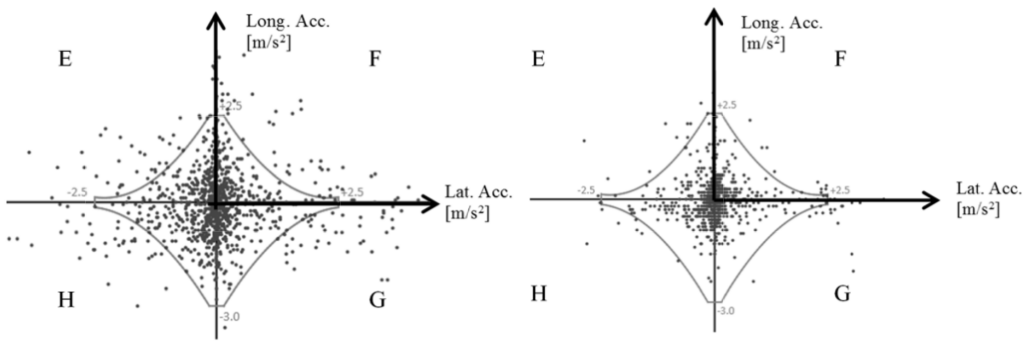
\includegraphics[scale=0.5]{10(2).png}
\caption{Distribución de puntos en el Diagrama de Estilo de Conducción para un conductor agresivo (izquierda) y uno conservador (derecha) (imagen tomada de \cite{vaiana2014driving}).}
\label{10(2)}
\end{figure}

En \cite{wu2013driving} se hace el prototipo de un dispositivo para el registro de eventos de conducción basado en el comportamiento al conducir, mediante el uso de herramientas como acelerómetros, cámaras y GPS.
Este dispositivo provee información acerca de siete comportamientos al conducir: conducción normal, aceleración, desaceleración, cambio al carril izquierdo o derecho, conducción en zigzag y aproximación al vehículo de enfrente.
El prototipo consiste en un arreglo de los componentes mencionados en forma de caja. 
Los resultados experimentales de este trabajo logran un promedio de $95\%$ de detección para el reconocimiento de comportamientos al conducir.

El trabajo realizado en \cite{6856461} trata sobre del desarrollo de una aplicación para teléfonos móviles, la cual detecta comportamientos de distracción a la hora de conducir, brindando las correspondientes observaciones a los conductores y alertándolos en caso de que su modo de conducir sea inseguro. 
La finalidad del desarrollo de esta aplicación es evitar accidentes automovilísticos, así como fomentar las prácticas de conducción seguras entre los usuarios. 
Las herramientas utilizadas para tales fines son sensores inerciales, GPS, cámaras y micrófonos. 
El proceso para lograr la detección comienza colocando el teléfono móvil justo debajo del espejo retrovisor, con la cámara apuntando hacia la carretera. 
Una vez hecho esto, la aplicación utiliza técnicas de reconocimiento de patrones con el fin de detectar los comportamientos de distracción más comunes en la conducción; tales como, cambiar de carril sin encender las luces intermitentes o la incapacidad del conductor para mantener el vehículo centrado en el carril correspondiente. 
Todo ello se logra al hacer uso de la información obtenida por la cámara y los sensores del teléfono, identificando automáticamente las líneas delimitadoras de los carriles y analizando el comportamiento del vehículo respecto a estas. 
La superación de umbrales de aceleración es otro de los factores importantes para la detección de tales comportamientos.

\begin{figure}[H]
\centering
\begin{tikzpicture}
  \node{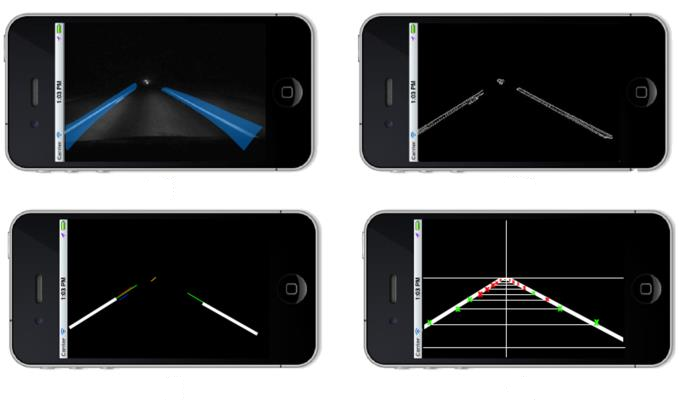
\includegraphics[scale=0.8]{12(2).png}};
  \node at (-3.6,.2) {$a)$};
  \node at (4,.2) {$b)$};
  \node at (-3.6,-4) {$c)$};
  \node at (4,-4) {$d)$};
\end{tikzpicture}
\caption{Proceso de detección de líneas en la noche: $a)$ Regiones de interés en escala de grises. $b)$ Límites de la carretera. $c)$ Líneas segmentadas y continuas. $d)$ Indicador de mediciones y modelado de camino (imagen tomada de \cite{6856461}).}
\label{12(2)}
\end{figure}

En \cite{6728289} se desarrolla un método que busca crear perfiles de comportamiento de conductores. 
También se trata de identificar eventos de conducción peligrosos, mediante el análisis de información recopilada por sensores en un vehículo. 
Para ello se recurre a la utilización de diferentes dispositivos incluidos en los teléfonos móviles: acelerómetro, GPS y magnetómetro. 
La información registrada al finalizar un recorrido común a bordo de un vehículo se envía a un servidor, en el cual se analizan los diferentes comportamientos de los conductores. 
Cada perfil de conducción se construye en base a 12 variables, medidas a lo largo de cada recorrido. 
Las cuales son utilizadas en un sistema de lógica difusa como el que se muestra en la tabla \ref{14(2)}, compuesto por 18 reglas, donde el resultado de cada una informa cual fue el tipo de conducción realizado de entre tres posibilidades: moderado, normal y agresivo. 

\begin{table}[H]
\centering
\begin{tabular}{c|c|c}
\hline \hline
\multicolumn{3}{p{10cm}}{\centering \bf Reglas de inferencia} \\ % p{ancho de texto}
\hline \hline 
No. & IF & THEN \\ \hline
1 & $OS_T=L\ \text{\fontfamily{qcr}\selectfont AND}\ OS_A=L\ \text{\fontfamily{qcr}\selectfont AND}\ OS_P=L$ & $NOR$\\ 
2 & $OS_T=M\ \text{\fontfamily{qcr}\selectfont AND}\ OS_A=M\ \text{\fontfamily{qcr}\selectfont AND}\ OS_P=M$ & $MOD$\\
3 & $OS_T=H\ \text{\fontfamily{qcr}\selectfont AND}\ OS_A=H\ \text{\fontfamily{qcr}\selectfont AND}\ OS_P=H$ & $AGG$\\
4 & $(SA_M=L\ \text{\fontfamily{qcr}\selectfont OR}\ SA_M=M)\ \text{\fontfamily{qcr}\selectfont AND}\ SA_A=L$ & $NOR$\\
5 & $(SA_M=M\ \text{\fontfamily{qcr}\selectfont OR}\ SA_M=H)\ \text{\fontfamily{qcr}\selectfont AND}\ SA_A=L$ & $MOD$\\
6 & $(SA_A=M\ \text{\fontfamily{qcr}\selectfont OR}\ SA_A=H)\ \text{\fontfamily{qcr}\selectfont AND}\ SA_M=H$ & $AGG$\\
7 & $(GA_M=L\ \text{\fontfamily{qcr}\selectfont OR}\ GA_M=M)\ \text{\fontfamily{qcr}\selectfont AND}\ GA_A=L$ & $NOR$\\
8 & $(GA_M=M\ \text{\fontfamily{qcr}\selectfont OR}\ GA_M=H)\ \text{\fontfamily{qcr}\selectfont AND}\ GA_A=L$ & $MOD$\\
9 & $(GA_A=M\ \text{\fontfamily{qcr}\selectfont OR}\ GA_A=H)\ \text{\fontfamily{qcr}\selectfont AND}\ GA_M=H$ & $AGG$\\
10 & $GA_P=L\ \text{\fontfamily{qcr}\selectfont AND}\ GA_N=L$ & $NOR$\\
11 & $GA_P=M\ \text{\fontfamily{qcr}\selectfont AND}\ GA_N=M$ & $MOD$\\
12 & $GA_P=H\ \text{\fontfamily{qcr}\selectfont AND}\ GA_N=H$ & $AGG$\\
13 & $(BR_M=L\ \text{\fontfamily{qcr}\selectfont AND}\ BR_M=M)\ \text{\fontfamily{qcr}\selectfont AND}\ BR_A=L$ & $NOR$\\
14 & $(BR_M=M\ \text{\fontfamily{qcr}\selectfont AND}\ BR_M=H)\ \text{\fontfamily{qcr}\selectfont AND}\ BR_A=L$ & $MOD$\\
15 & $(BR_A=M\ \text{\fontfamily{qcr}\selectfont AND}\ BR_A=H)\ \text{\fontfamily{qcr}\selectfont AND}\ BR_M=H$ & $AGG$\\
16 & $BR_P=L$ & $NOR$ \\
17 & $BR_P=M$ & $MOD$ \\
18 & $BR_P=H$ & $AGG$ \\
\hline \hline
\end{tabular}
\caption{Lista de reglas de inferencia (tabla tomada de \cite{6728289}).}
\label{14(2)}
\end{table}

La forma en que los autores evalúan el comportamiento del conductor es asignándole una puntuación a cada una de las salidas. 
Las cuales son sometidas a una serie de operaciones, dando como resultado una puntuación final entre $0$ y $100$, siendo $0$ la mejor y $100$ la peor.

Usando métodos similares a los explicados en \cite{6728289}, tales como sistemas de lógica difusa, los autores de \cite{7014406} desarrollan una plataforma que utiliza el acelerómetro, GPS, magnetómetro y sensor de gravedad incluidos en los teléfonos móviles. Esto con el propósito de registrar información durante el trayecto de un vehículo, la cual servirá para crear un perfil de conducción para cada usuario. 
También buscan ofrecer información sobre eventos de riesgo individual de los conductores, así como de la rapidez y manejo ecológico del vehículo. 
Una de las características que distingue a este trabajo de otros similares es el uso de información sobre condiciones climáticas como factor para determinar los eventos de riesgo. 
Dentro de los eventos de riesgo, los autores intentan detectar exceso de velocidad, aceleración, frenado y direccionamiento. 
Mediante notificaciones sonoras y gráficas en el teléfono móvil se alerta al usuario sobre la ocurrencia de alguno de estos eventos.

En \cite{7338354} se tiene el propósito de realizar un monitoreo detallado de los comportamientos anormales en la conducción de automóviles, dando la retroalimentación correspondiente a los conductores; para lo cual se realiza una recopilación de datos de conducción en ambientes reales durante seis meses. 
Los autores identifican seis tipos de comportamientos anómalos de conducción: movimiento trenzado, desviación, deslizamiento, movimiento en U rápido, giro de amplio radio y frenado repentino.
Estos son detectados al aplicar técnicas de aprendizaje automático a los datos obtenidos, para ello se establecen 16 características representativas que pueden identificar a cada uno de los seis comportamientos de conducción. 
Tales características constan de diferentes parámetros de aceleración, orientación, tiempo de ejecución de los eventos, entre otros; los cuales son determinados a partir de las mediciones de los sensores. 
Complementariamente, se estima el impacto de diferentes factores sobre el desempeño de la plataforma, tales como condiciones de tráfico, tipo de carretera, lugar de colocación del teléfono, entre otros.

En \cite{Hong:2014:SSP:2611222.2557321} se propone la implementación de una plataforma de medición, con la cual se pretende realizar una valoración y evaluación automática del estilo de conducción. 
La plataforma hace uso de los sensores incluidos en teléfonos móviles, dispositivos para el diagnóstico del vehículo y técnicas de aprendizaje automático. 
La metodología empleada para la evaluación requiere de la información de un cierto número de características relativas a la conducción, las cuales se encuentran en la diversa información recolectada. 
Dicha información está compuesta por datos de velocidad, aceleración, desaceleración, revoluciones por minuto del motor, posición del acelerador y dirección del movimiento de las ruedas. 
Los autores tienen como objetivo que en el futuro se puedan identificar estilos de conducción agresivos en tiempo real, así como proveer la retroalimentación pertinente al conductor, con el fin de mejorar el estilo de conducción de los usuarios. 

Haciendo un resumen de los trabajos presentados en este capítulo, se puede destacar la gran cantidad de aplicaciones para teléfonos móviles, desarrolladas con fines de prevención de conductas incorrectas en la conducción.
Lo cual es debido principalmente a la masificación y disminución en los costos de dispositivos como las IMU's.
Tal accesibilidad en estos dispositivos también ha dado lugar al desarrollo de soluciones en diferentes ámbitos de la conducción de vehículos, las cuales no están necesariamente enfocadas en automóviles, sino en vehículos como bicicletas o trenes.

Las metodologías empleadas para la detección de diferentes conductas en los pilotos, así como de movimientos anormales en los distintos medios de transporte analizados son muy variadas; van desde análisis en la dinámica de los vehículos en tiempo real, hasta el uso de electroencefalogramas para estudios del comportamiento de los usuarios a la hora de conducir.
Sin embargo, en la investigación realizada de los trabajos relacionados, se encontró que estos utilizan mayoritariamente el estudio de la dinámica a diferentes niveles, junto con umbrales de aceleración y/o velocidad predefinidos; o bien, sistemas muy sofisticados con multiples sensores para la determinación de conducciones anómalas.
La propuesta que se realiza en este trabajo difiere de las presedentes en que no se basa en el estudio de la dinámica propia del vehículo, además de que solo requiere de un dispositivo IMU como sensor.
En el siguiente capítulo se detallarán las bases teóricas y componentes de hardware utilizados para este trabajo.
